% =========================================================================== %
% Yes. This is a document.

\documentclass[
	english,
	aspectratio=169,
	table
]{beamer}

% =========================================================================== %
% Theme
\usepackage{scrlfile}
	\ReplacePackage{beamerthemeSHUR}{./sty/beamerthemeSHUR}
	\ReplacePackage{beamerinnerthemefancy}{./sty/beamerinnerthemefancy}
	\ReplacePackage{beamerouterthemedecolines}{./sty/beamerouterthemedecolines}
	\ReplacePackage{beamercolorthemechameleon}{./sty/beamercolorthemechameleon}

\usetheme[
	pageofpages=/,
	bullet=circle,
	titleline=true,
	alternativetitlepage=true,
	watermark="",
	watermarkheight=0px,
	watermarkheightmult=0
	]
{SHUR}

% =========================================================================== %
% the usual stuff

\usepackage[utf8]{inputenc}
\usepackage[T1]{fontenc}
\usepackage{babel}
\usepackage{lmodern}
\usepackage{microtype}
\usepackage{csquotes}
\usepackage{xspace}

\usepackage{tabularx}
\usepackage{booktabs}
\usepackage{multirow}

\usepackage{color, colortbl}
\usepackage{xcolor}
	\definecolor{tabhighlight}{RGB}{230,240,255}

\usepackage{tabto}

\usepackage{minted}
	\usemintedstyle{friendly}

\usepackage{tikz}
	\usetikzlibrary{positioning}
	\usetikzlibrary{matrix}
	\usetikzlibrary{shapes.geometric}
	\usetikzlibrary{backgrounds}
	\usetikzlibrary{calc}
	\usetikzlibrary{decorations.pathreplacing}
	\tikzstyle{every picture}+=[remember picture] 
\usepackage{adjustbox}

\usepackage{amsmath}
\usepackage{physics}

\usepackage[most]{tcolorbox}
	\tcbsetforeverylayer
		{colback=cyan!10!white,
		 colframe=cyan!75!black,
		 arc=0pt,
		 outer arc=0pt
		}
	\newtcolorbox{codebox}[1][Code]
		{colback=black!5!white,
		 colframe=blue!40!black,
		 title=#1,
		 leftupper=6mm
		}
	\newtcolorbox{cmdbox}[1][Command Line]
		{colback=black,
		 coltext=white,
		 fontupper=\ttfamily ,
		 colframe=blue!40!black,
		 title=#1,
		 outer arc=0pt
		}
	\newtcolorbox{warnbox}[1][Warning]
		{colback=black!5!white,
		 colframe=red!40!black,
		 title=#1
		}
	\newtcolorbox{hintbox}[1][Hint]
		{colback=black!5!white,
		 colframe=green!40!black,
		 title=#1
		}
	\newtcolorbox{defbox}[1][Code]
		{colback=cyan!10!white,
		 colframe=cyan!90!black,
		 title=#1
		}
	\newtcolorbox{recapbox}[1][Code]
		{colback=yellow!10!white,
		 colframe=yellow!90!black,
		 coltitle=black,
		 title=#1
		}
%==============================================================================%
% GLOBAL MACROS

\newcommand*{\zB}{e.\,g. }
\newcommand*{\ie}{i.\,e. }

\newcommand{\Thus}{\ensuremath{\Rightarrow}\xspace}
\newcommand{\thus}{\ensuremath{\rightarrow}\xspace}

\newcommand*{\tabcrlf}{\\ \midrule}			% actually still allows for optional argument

\newcommand*{\inPy}[1]{\mintinline{python}{#1}}

\newcommand*{\todo}[1]{{\color{red}TODO: #1}}
\newcommand*{\sfrac}[2]{\ensuremath{{}^{#1}/_{#2}}}

% =========================================================================== %

\author{Stefan Hartinger}
\title{Python for Scientists}
\subtitle{Part 19: Regular Expressions}
\institute{Department of Just Some Dude Who Likes to Talk}
\date{Winter 2023/24}

% =========================================================================== %

\begin{document}
\newcommand{\rx}[1]{\texttt{"{\color{olive}#1}"}}
\newcommand{\match}[1]{{\color{blue}#1}}
\newcommand{\qtt}[1]{\texttt{"{#1}"}}

% =========================================================================== %

\begin{frame}[t,plain]
\titlepage
\end{frame}

% =========================================================================== %

\begin{frame}[fragile]{Regular Expressions}
%
\begin{center}
\begin{columns}
\column{.45\linewidth}
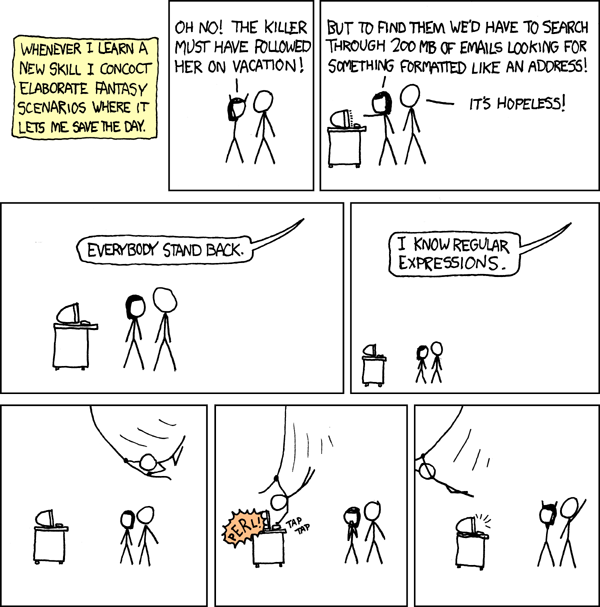
\includegraphics[width=\linewidth]{./gfx/19-xkcd-regular_expressions}
%
\column{.45\linewidth}
\emph{Wait, forgot to escape a space.} \\
\emph{Wheeeeee[taptaptap]eeeeee.}

\vspace{6pt}
Source: \url{https://xkcd.com/208/}

\begin{hintbox}[Perl]
\footnotesize
Perl is a high-level, general-purpose, interpreted, dynamic programming language%
\footnote{\tiny\url{https://en.wikipedia.org/wiki/Perl}}
that looks the same before and after compiling%
\footnote{\tiny\url{https://dev.to/thibaultduponchelle/the-hate-of-perl-in-memes-469e}}%
.
\end{hintbox}
\end{columns}
\end{center}
%
\end{frame}

% =========================================================================== %

\begin{frame}{Scope For Today}
%
\begin{itemize}
\item Regular Expressions
	\begin{itemize}
	\item Concept and Use Case
	\item Patterns
	\item Numbered and Named Groups
	\end{itemize}
\item Python's \texttt{re} package
	\begin{itemize}
	\item Matching Strings and Replacing Substrings
	\item Some Examples
	\end{itemize}
\end{itemize}
%
\end{frame}

% =========================================================================== %

\begin{frame}{Concept and Use Case}
%
\begin{itemize}
\item Regular Expression (aka RegEx or RE)
	\begin{itemize}
	\item A String describing the \emph{structure} of another string
	\item E.\;g.: groups of three digits separated by a hyphen
	\item Expressed by a computer-readable syntax
	\end{itemize}
\pause
\item More powerful form of \emph{search string with wildcards}: Concepts like
	\begin{itemize}
	\item \emph{must begin/end with}
	\item \emph{must be preceded/followed by}
	\item \emph{words longer than N characters}
	\item \emph{must contain between N and M repetitions}
	\item Find position(s) of matches, if any
	\end{itemize}
\pause
\item Supported in many programming languages
	\begin{itemize}
	\item Python: Built-in package \texttt{re}
	\item C++: stdlib header \texttt{regex} in \texttt{c++11} and higher
	\item C: POSIX libararies (\texttt{regex.h})
	\item Groovy, Perl, Ocaml, Julia: built in
	\end{itemize}
\end{itemize}
%
\end{frame}

% =========================================================================== %

\begin{frame}{Basic Structure of a RE}
%
\begin{itemize}
\item Arbitrary String \emph{without special characters}
	\begin{itemize}
	\item Interpret as: \emph{look for this substring anywhere in the search string}
	\end{itemize}
\item Special characters
	\vspace{-9pt}
	\begin{columns}[T]
	\column{.4\linewidth}
	\begin{itemize}
	\setlength\itemsep{-2pt}
	\item Parens \texttt{()}
	\item Braces \texttt{\{\}}
	\item Brackets \texttt{[]}
	\item Backslash \texttt{\textbackslash}
	\item Dot \texttt{.}
	\item Pipe Symbol \texttt{|}
	\end{itemize}
	\column{.4\linewidth}
	\begin{itemize}
	\setlength\itemsep{-2pt}
	\item Caret \texttt{\textasciicircum}
	\item Dollar Sign \texttt{\$}
	\item Plus \texttt{+}
	\item Asterisk \texttt{*}
	\item Question Mark \texttt{?}
	\end{itemize}
	\end{columns}
\end{itemize}
%
\begin{hintbox}[Dialects of Regular Expressions]
\footnotesize
There are dozends of RE engines, and they do not agree on all details of syntax.\\
Below, we focus on the Python \texttt{re} dialect. You may need to rewrite your REs when porting to another language.
Most of the concepts should be available, though.
\end{hintbox}
%
\end{frame}

% =========================================================================== %

\begin{frame}[fragile]{Examples}
%
\begin{tcbraster}[raster columns=2,
                  raster equal height,
                  nobeforeafter,
                  raster column skip=0.1cm]
\begin{codebox}[Pattern]
\rx{foo bar}
\end{codebox}
%
\begin{codebox}[Matches]
\qtt{Your foo-\match{foo bar}ely meets the minimum requirements.}
\end{codebox}
\end{tcbraster}
%
\vspace{-9pt}
\begin{tcbraster}[raster columns=2,
                  raster equal height,
                  nobeforeafter,
                  raster column skip=0.1cm]
\begin{codebox}[Pattern]
\rx{aa}
\end{codebox}
%
\begin{codebox}[Matches]
\qtt{A\match{aa}aah!}\\
\qtt{Aa\match{aa}ah!}\\
\qtt{Aaa\match{aa}h!}
\end{codebox}
\end{tcbraster}
%
\vspace{-9pt}
\begin{hintbox}[Overlapping Matches]
\footnotesize
Due to implementation details, it is difficult to actually obtain the second match. Only non-overlapping matches are easy to fetch. Still, technically all three of them constitute matches.
\end{hintbox}
%
\end{frame}

% =========================================================================== %

\begin{frame}{Matching Special Characters and Nested Escape Sequences}
%
\begin{itemize}
\item To match any of the special characters: prepend them with a backslash
	\begin{itemize}
	\item[\Thus] \rx{This matches an {\color{purple}\textbackslash*} asterisk.}
	\end{itemize}
\pause
\item But: Python uses the same escape character!
	\begin{itemize}
	\item[\Thus] You need to type \rx{This matches an {\color{purple}\textbackslash\textbackslash*} asterisk.}
	\item[\Thus] You need to type \rx{This matches a {\color{purple}\textbackslash\textbackslash\textbackslash\textbackslash} backslash.}
	\end{itemize}
\pause
\item Best practice: use Python raw strings
	\begin{itemize}
	\item Prepend string with an \texttt{r}
	\item [\Thus] You need to type \texttt{{\color{purple}r}"{\color{olive}This matches an {\color{purple}\textbackslash*} asterisk.}"}
	\item [\Thus] You need to type \texttt{{\color{purple}r}"{\color{olive}This matches an {\color{purple}\textbackslash\textbackslash} backslash.}"}
	\end{itemize}
\end{itemize}
%
\pause
\begin{hintbox}[More Escape Sequences]
\footnotesize
The backslash offers more functionality than only escaping special characters. We will cover this after discussing the special characters themselves.
\end{hintbox}
%
\end{frame}

% =========================================================================== %

\begin{frame}{Using Wildcards}
%
\begin{itemize}
\item A dot (\texttt{.}) matches any character except for newline	(\texttt{\textbackslash n})
	\begin{itemize}
	\item Matches exactly one arbitrary character
	\item[\Thus] \rx{a.} matches \qtt{\match{aa}}, \qtt{\match{a1}} and \qtt{\match{a }}
	\item[\Thus] \rx{a.} does not match \qtt{a} or \qtt{a{\color{red}\textbackslash{}n}x}
	\end{itemize}
\pause
\item An asterisk (\texttt{*}) modifies the previous RegEx element to match arbitrary many repetitions
	\begin{itemize}
	\item[\Thus] \rx{.*} matches \emph{any string}, including the \emph{null string}
	\item[\Thus] \rx{x.*y} matches \qtt{\match{xy}}, \qtt{\match{xzy}} and \qtt{\match{xabcy}}
	\item[\Thus] \rx{foo*} matches \qtt{\match{fo}}, \qtt{\match{foo}} and \qtt{\match{fooooooo}}
	\end{itemize}
\pause
\item A plus (\texttt{+}) works like the asterisk, but must match at least once
	\begin{itemize}
	\item[\Thus] \rx{foo+} matches \qtt{\match{foo}} and \qtt{\match{foooooo}}, but not \qtt{fo} 
	\end{itemize}
\item A question mark (\texttt{?}) matches zero or one occurences.
\pause
\item Parens () combine RegEx elements into \emph{groups}
	\begin{itemize}
	\item \rx{(foo)*} matches \qtt{\match{foo}}, \qtt{\match{foofoo}} and \qtt{}
	\item \rx{({\color{purple}.\{2\}})*} matches \qtt{{\color{blue}abcd}e}
	\end{itemize}
\end{itemize}
%
\end{frame}

% =========================================================================== %\\

\begin{frame}{Specified Number of Repetitions and Greediness}
%
Braces can be used to specify the number of repetitions
\begin{itemize}
\item \rx{a\{\textit{n}\}} matches exactly $n$ occurrences of \rx{a}
	\begin{itemize}
	\item \texttt{a} is an arbitrary RegEx element, including \emph{groups}
	\item[\Thus] \rx{fo\{2\}} matches \qtt{\match{foo}} but not \qtt{fo}. In \qtt{\match{foo}o}, only the blue part is matched.
	\end{itemize}
\pause
\item \rx{a\{\textit{n},\textit{m}\}} matches between $n$ and $m$ occurrences of \rx{a}
	\begin{itemize}
	\item If $n$ is ommitted, assume $0$
	\item If $m$ is ommitted, assume $\infty$
	\item[\Thus] \rx{fo\{2,4\}} matches 
		\qtt{\match{foo}},
		\qtt{\match{foooo}} 
		and the blue part in 
		\qtt{\match{foooo}oo},
		but not 
		\qtt{fo}
	\item[\Thus] \rx{fo\{2,\}} is equivalent to \rx{foo+}
	\item[\Thus] \rx{fo\{,2\}} matches 
		\qtt{\match{f}},
		\qtt{\match{fo}},
		\qtt{\match{foo}} 
		and the blue part in 
		\qtt{\match{foo}oo}
	\end{itemize}
\end{itemize}
\pause

By default, repetition markers are \emph{greedy}
\begin{itemize}
\item Match longest substring
	\begin{itemize}
	\item \rx{fo*} matches all of \qtt{\match{fooooooo}}, not only \qtt{\match{f}ooooooo} (or any smaller number of \texttt{o}'s)
	\item \rx{fo\{2,5\}} matches \qtt{\match{fooooo}oo} even though \qtt{\match{foo}ooooo} appears legit, too
	\item \rx{fo\{,2\}o} matches \qtt{\match{foo}} due to a backtracking mechanism
	\end{itemize}
\end{itemize}
%
\end{frame}

% =========================================================================== %

\begin{frame}{Modifying Greedy Behaviour}
%
\begin{itemize}
\item By default, repetition markers attempt to match the longest substring
	\begin{itemize}
	\item E.\;g. \rx{<.*>} matches \qtt{\match{<a> b <c>}} and not only \qtt{\match{<a>} b <c>}
	\end{itemize}
\pause
\item A questionmark (\texttt{?}) can be prepended to all variable size repetition markers 
	\begin{itemize}
	\item That includes \texttt{*?}, \texttt{+?}, \texttt{??}, \texttt{\{\textit{n}, \textit{m}\}?}
	\item This deactivates the greedy behaviour
	\item E.\;g. \rx{<.*{\color{purple}?}>} matches only \qtt{\match{<a>} b <c>}
	\end{itemize}
\pause
\item A plus (\texttt{+}) can be prepended to keep greediness but deactivate backtracking
	\begin{itemize}
	\item That includes \texttt{*+}, \texttt{++}, \texttt{?+}, \texttt{\{\textit{n}, \textit{m}\}+}
	\item E.\;g. \rx{fo\{,2\}{\color{purple}+}o} does not match \qtt{foo}
		\begin{itemize}
		\item \rx{fo\{,2\}{\color{purple}+}} already matches \qtt{\match{foo}}
		\item The \texttt{\color{purple}+} forbids giving up the matched \texttt{\color{blue}o}'s for the next RegEx elements
		\item There is nothing left in the search string to match the remaining \rx{o}
		\end{itemize}
	\end{itemize}
\end{itemize}
%
\end{frame}

% =========================================================================== %

\begin{frame}{Character Sets}
%
\begin{itemize}
\item Brackets define \emph{sets}: they list individual allowed characters
	\begin{itemize}
	\item \rx{[amc]\color{purple}+} matches \qtt{St\match{ac}y's \match{ma}n \match{ca}n} (in three separate results)
	\item \rx{[amc]\color{purple}*} additionally matches null strings for any otherwise unmatched character in the search string
	\end{itemize}
\pause
\item Special characters lose their special meaning inside sets. 
	\begin{itemize}
	\item \rx{[(*+)]} matches any of \qtt{\match{(}}, \qtt{\match{*}}, \qtt{\match{+}} or \qtt{\match{)}}
	\end{itemize}
\pause
\item Exception: A caret (\texttt{\textasciicircum}) as first character in the set turns it into an \emph{exclusion set}
	\begin{itemize}
	\item \rx{[\textasciicircum X]+} matches \texttt{\match{An\underline{~}}X\match{\underline{~}marks\underline{~}the\underline{~}spot}} (in two separate results)
	\item \rx{[\textasciicircum\textasciicircum]} matches anything but the caret
	\end{itemize}
\pause
\item Characters with consecutive code points (think: ASCII codes) can be denoted in a \emph{from...to} notation with a hyphen
	\begin{itemize}
	\item \rx{[a-z]} matches any lower case letter
	\item \rx{[0-9A-Fa-f]} matches any hexadecimal digit
	\end{itemize}
\item Backslash can be used to escape the hyphen
	\begin{itemize}
	\item \rx{[A\textbackslash-Z]} matches \qtt{Uppercase Letters Not Matched But Hyphen \match{-}.}
	\end{itemize}
\end{itemize}
%
\end{frame}

% =========================================================================== %

\begin{frame}{Referencing Partial Matches}
%
\begin{itemize}
\item \emph{Groups} (anything in parens \texttt{()}) are cached and numbered
	\begin{itemize}
	\item A matched group can be referenced in a pattern by using \texttt{\textbackslash\textit{number}}
	\item \texttt{\textit{number}} is the number of the group in the pattern, starting at 1
	\item[\Thus] \rx{({\color{purple}.+})-{\color{purple}\textbackslash 1}} matches \qtt{Ding-\match{Dong-Dong}!}
	\end{itemize}
\pause
\item \emph{Groups} can be named to get \emph{slightly} better readable patterns
	\begin{itemize}
	\item Use \rx{(?P<\textit{name}>\textit{pattern})} to assign the name \texttt{\textit{name}} to the pattern \texttt{\textit{pattern}}
	\item Use \rx{(?P=\textit{name})} to refer back to the previously matched group
	\item Named groups must be unique within one pattern (no redefinition)
	\item[\Thus] \rx{({\color{teal}?P<quote>}{\color{purple}['"]}).*?({\color{teal}?P=quote})} matches any quoted string, with either single \emph{or} double quotes.
	\end{itemize}
\pause
\item Remember to use raw strings (\inPy{r"\1"}) or to escape the backslash itself (\inPy{"\\1"}) in numbered group references!
\end{itemize}
%
\end{frame}

% =========================================================================== %

\begin{frame}{Lookahead- and Lookback-Assertion}
%
\begin{itemize}
\item You can tie matches to secondary conditions
	\begin{itemize}
	\item Match <pattern> only, if preceded/followed by <other pattern>
	\item Only <pattern> will be in the results, but not <other pattern>
	\end{itemize}
\pause
\item Lookahead Assertion: \rx{(?=\textit{other pattern})}
	\begin{itemize}
	\item[\Thus] \rx{Isaac (?=Asimov)} matches \qtt{While \match{Isaac\underline{~}}Asimov wrote fiction, Isaac Newton was a scientist.}
	\end{itemize}
\item Lookback Assertion: \rx{(?<=\textit{other pattern})}
	\begin{itemize}
	\item[\Thus] \rx{(?<=Isaac )Asimov} matches \qtt{Isaac \match{Asimov} had two siblings: Marcia Asimov and Stanley Asimov.}
	\end{itemize}
\pause
\item There are also negative forms (only match, if <other pattern> is not found)
	\begin{itemize}
	\item Negative lookahead assertion: \rx{(?!\textit{other pattern})}
	\item Negative lookback assertion: \rx{(?<!\textit{other pattern})}
	\end{itemize}
\end{itemize}
%
\end{frame}

% =========================================================================== %

\begin{frame}{Predefined Patterns}
%
\begin{itemize}
\item \rx{\textbackslash d} matches any decimal digit. Roughly equivalent to \rx{[0-9]}, but extra rules for unicode characters
\item \rx{\textbackslash D} matches any \emph{non} decimal digit.
\pause
\vspace{6pt}
\item \rx{\textbackslash s} matches any whitespace character. Roughly equivalent to \rx{[ \textbackslash t\textbackslash n\textbackslash r\textbackslash f\textbackslash v]}
\item \rx{\textbackslash S} matches any \emph{non} whitespace character
\pause
\vspace{6pt}
\item \rx{\textbackslash w} matches any word characters. Roughly equivalent to \rx{[a-zA-Z0-9\_]}
\item \rx{\textbackslash W} matches any \emph{non} word character
\pause
\vspace{6pt}
\item \rx{\textbackslash b} matches a word boundary, 
	\ie either an empty string between a \rx{\textbackslash w} and a \rx{\textbackslash W} character, 
	or an empty string at the beginning/end of the string
	\begin{itemize}
	\item Use this to match \emph{something at the beginning/end of a word}
	\end{itemize}
\item \rx{\textbackslash B} matches an empty string within a word
\end{itemize}
%
\end{frame}

% =========================================================================== %

\begin{frame}{Miscellaneous}
%
\begin{itemize}
\item The caret (\texttt{\textasciicircum}) matches the begin of the string
	\begin{itemize}
	\item Used alone, it matches the empty string
	\item[\Thus] \rx{\textasciicircum foo} matches \qtt{\match{foo} bar} but not \qtt{{\color{red}Fee fie }foo!}
	\end{itemize}
\item The dollar sign (\texttt{\$}) matches the end of the string
	\begin{itemize}
	\item Likewise, alone it matches an empty string
	\item[\Thus] \rx{foo\$} matches \qtt{foo-\match{foo}} but not \qtt{foo-foo\color{red}!}
	\end{itemize}
\pause
\item The pipe symbol (\texttt{|}) acts like a logical \emph{or}
	\begin{itemize}
	\item Evaluated lazily: if in \rx{A|B}, \rx{A} matches, then \rx{B} is never checked
	\item[\Thus] \rx{(Music)|(Coding)} matches \qtt{\match{Coding} is fun!}
	\item[\Thus] \rx{(Python)|(Perl)} matches \qtt{Both, \match{Python} and Perl support Regular Expressions}
	\end{itemize}
\pause
\item Still more features
	\begin{itemize}
	\item Look for yourself at \url{https://docs.python.org/3/library/re.html}
	\end{itemize}
\end{itemize}
%
\end{frame}

% =========================================================================== %

\begin{frame}{The Python Package \texttt{re}}
%
\begin{itemize}
\item Built-in package \texttt{re}
\item Provides classes \texttt{Pattern}, \texttt{Match} and exception \texttt{error}
	\begin{itemize}
	\item \texttt{Pattern}: pattern string, translated into internal format for easier handling of the task
	\item \texttt{Match}: representation of the match, \ie contains information where what was found
	\item \texttt{error}: \inPy{raise}d when a pattern string is malformed
	\end{itemize}
\pause
\item Recommended usage
	\begin{itemize}
	\item \inPy{import re}
	\item \inPy{pattern = re.compile(pattern_string)}
	\item Different methods on \texttt{pattern} for actual matching operation
		\begin{itemize}
		\item E.\;g. \inPy{match = pattern.search(search_string)}
		\item Extract match data via methods like \texttt{match.start()}, \texttt{match.end()}
		\item More on the next slides
		\end{itemize}
	\end{itemize}
\pause
\item Alternative (less efficient)
	\begin{itemize}
	\item \inPy{match = re.match(pattern_string, search_string)}
	\item Okay for single use; needs to be recompiled when \texttt{pattern\_string} used more often
	\item Actually buffered, but still causes lookup overhead
	\end{itemize}
\end{itemize}
%
\end{frame}

% =========================================================================== %

\begin{frame}{The \texttt{Pattern} Class in Detail (1)}
%
\begin{itemize}
\item \inPy{pattern.search(search_string, pos=0, endpos=2**64-1)}
	\begin{itemize}
	\item Looks for pattern anywhere in \texttt{search\_string}
	\item Can be limited to a substring with the \texttt{pos} and \texttt{endpos} optional arguments
	\item Finds only first \texttt{Match} in that range
	\item Retruns \inPy{None} if no match (Note: this is different from an empty \texttt{Match})
	\end{itemize}
\pause
\item \inPy{pattern.match(search_string, pos=0, endpos=2**64-1)}
	\begin{itemize}
	\item Same as \texttt{search}, but only matches if \texttt{pattern} matches with start of \texttt{search\_string}
	\item Equivalent to \texttt{search} with \rx{\textasciicircum\textit{pattern\_string}}
	\end{itemize}
\pause
\item \inPy{pattern.fullmatch(search_string, pos=0, endpos=2**64-1)}
	\begin{itemize}
	\item Same as \texttt{search}, but requires entire string to match
	\item Equivalent to \texttt{search} with \rx{\textasciicircum\textit{pattern\_string}\$}
	\end{itemize}
\end{itemize}
%
\end{frame}

% =========================================================================== %

\begin{frame}{The \texttt{Pattern} Class in Detail (2)}
%
\begin{itemize}
\item \inPy{pattern.finditer(search_string, pos=0, endpos=2**64-1)}
	\begin{itemize}
	\item Finds all \emph{non overlapping} \texttt{Match}es and returns an Iterator over them
	\item[\Thus] You can write \inPy{for match in pattern.finditer(search_string): ...}
	\item[\Thus] With \rx{aa} in \qtt{A\match{aa}{\color{purple}aa}h!}, you will get only \emph{two} \texttt{Match}es.
	\end{itemize}
\pause
\item \inPy{pattern.findall(search_string, pos=0, endpos=2**64-1)}
	\begin{itemize}
	\item Finds all \emph{non overlapping} \texttt{Match}es and returns a \inPy{list} of all matching substrings
	\item You cannot retrieve the positions with this function
	\end{itemize}
\pause
\item \inPy{pattern.split(search_string, maxsplit=0)}
	\begin{itemize}
	\item Splits the text into a \inPy{list} of substrings; pplit points are matches
	\item Split into at most \texttt{maxsplit + 1} parts
	\item Groups will be included in the result
	\item Example: \rx{\textbackslash W+} on \qtt{Words, words, words.}
		\begin{itemize}
		\item Matches \qtt{Words\match{,\underline{~}}words\match{,\underline{~}}words\match{.}}. Returns \inPy{["Words", "words", "words", ""]}
		\end{itemize}
	\item Example: \rx{{\color{purple}(}\textbackslash W+{\color{purple})}} on \qtt{Words, words, words.}
		\begin{itemize}
		\item Same Matches. Returns \inPy{["Words", ", ", "words", ", ", "words", "."]}
		\end{itemize}
	\end{itemize}
\end{itemize}
%
\end{frame}

% =========================================================================== %

\begin{frame}[fragile]{Tangent: Python \inPy{str}ing Methods \texttt{split}, \texttt{rsplit} and \texttt{join}}
%
\begin{itemize}
\item \inPy{some_string.split(sep, maxsplit)} almost the same as \inPy{re.split(sep, some_string, maxsplit)}
	\begin{itemize}
	\item No pattern matching, but good enough for most cases
	\item If \texttt{sep} omitted: any whitespace character
	\item If \texttt{maxsplit omitted}: split all
	\end{itemize}
\pause
\item Analogous: \inPy{some_string.rsplit(sep = ",", maxsplit = -1)}
	\begin{itemize}
	\item Splits \enquote{from the right}
	\item Same order of elements
	\item E.\;g.: \inPy{"a b\tc d".rsplit(maxsplit=2)} yields \inPy{["a b", "c", "d"]}
	\end{itemize}
\pause
\item \inPy{joiner_string.join(iterable)}
	\begin{itemize}
	\item Transforms \inPy{joiner_string = "-"} and \inPy{iterable = ["1","2","3"]} into \inPy{"1-2-3"}
	\item Optimized to avoid repeated copying, thus \emph{much} faster than doing this manually (\inPy{buffer += next_part})
	\end{itemize}
\end{itemize}
%
\end{frame}

% =========================================================================== %

\begin{frame}{The \texttt{Pattern} Class in Detail (3)}
%
\begin{itemize}
\item \inPy{pattern.sub(repl, search_string, count=0)}
	\begin{itemize}
	\item Find all matches in \texttt{search\_string} and replaces them according to \texttt{repl}
	\item Number of replacements can be limited to \texttt{count}
	\end{itemize}
\pause
\item If \texttt{repl} is a \inPy{str}ing ...
	\begin{itemize}
	\item ... \emph{backslash processing} is performed
	\item Patterns like \texttt{\textbackslash n} are replaced by their proper characters (even in raw strings like \inPy{r"raw string"})
	\item Group references are resolved (\inPy{r"\1"} becomes whatever the first group matched)
	\end{itemize}
\pause
\item If \texttt{repl} is a \texttt{callable} ...
	\begin{itemize}
	\item ... \texttt{repl(m)} is called for each match
	\item Input parameter: \texttt{Match}
	\item Return value: \inPy{str}ing
	\end{itemize}
\end{itemize}
%
\end{frame}

% =========================================================================== %

\begin{frame}{The \texttt{Match} Class in Detail (1)}
%
\begin{itemize}
\item Most simple use: methods to retrieve match description
	\begin{itemize}
	\item \inPy{m.start()} -- index of the first matched character in the search string
	\item \inPy{m.end()} -- index of the last matched character in the search string
	\item \inPy{m[i]} -- the \texttt{i}$^{\text{th}}$ group
		\begin{itemize}
		\item Group 0 is the entire match
		\item Also works with named groups (\texttt{i} need not be an \inPy{int})
		\end{itemize}
	\item[\Thus] \inPy{m = re.search("aa", "Aaaaah!")} \thus \texttt{m.start() == 1}, \texttt{m.end() == 3}
	\item[\Thus] \inPy{m = re.search("(a)(b)", "ab")} \thus \texttt{m[0] == "ab"}, \texttt{m[1] == "a"}, \texttt{m[2] == "b"}
	\end{itemize}
\pause
\item Truthiness
	\begin{itemize}
	\item Result when converting to a \inPy{bool}ean (as per \inPy{__bool__})
	\item Always \inPy{True}
	\item Remember: \texttt{pattern.search} et al return \inPy{None} if nothing matched
	\item \inPy{None} has truthiness \inPy{False}
	\item[\Thus] You can write:
		\begin{itemize}
		\item \inPy{m = pattern.search(search_string)}
		\item \inPy{if m : print("matches pattern!")}
		\end{itemize}
	\end{itemize}
\end{itemize}
%
\end{frame}

% =========================================================================== %

\begin{frame}{The \texttt{Match} Class in Detail (2)}
%
\begin{itemize}
\item \texttt{m.groups()} -- returns all group values as \inPy{tuple} of \inPy{str}ings
	\begin{itemize}
	\item[\Thus] \inPy{re.match(r"(\d+)\.(\d+)", "24.1632").groups()} \thus \inPy{('24', '1632')}
	\end{itemize}
\pause
\item \texttt{m.groupdict()} -- same for named groups
	\begin{itemize}
	\item [\Thus] \inPy{m = re.match(r"(?P<first>\w+) (?P<last>\w+)", "Malcolm Reynolds")} \\
	              \inPy{m.groupdict()} \thus \inPy{{'first': 'Malcolm', 'last': 'Reynolds'}}
	\end{itemize}
\pause
\item \texttt{m.start()} and \texttt{m.end()} optionally take a \texttt{groupID} parameter, too
\item \texttt{m.span()} returns a \inPy{tuple} \texttt{(m.start(), m.end())} and takes an optional \texttt{groupID} parameter, too
\pause
\item \emph{Attribute} \texttt{lastindex} gives number of last matched group (or \inPy{None})
	\begin{itemize}
	\item[\Thus] Can be used to iterate over all groups
	\end{itemize}
\pause
\item \texttt{m.expand(template)} performs backslash substitutions in \inPy{str}ing \texttt{template}
	\begin{itemize}
	\item This includes group references
	\end{itemize}
\end{itemize}
%
\end{frame}

% =========================================================================== %

\begin{frame}{Tweaking the Matching Behaviour}
%
\begin{itemize}
\item \inPy{re.compile(pattern, flags = 0)} -- optional parameter
\item Predefined symbols that can be added together
\item E.\;g.: \inPy{re.compile(pattern, flags = re.IGNORECASE + re.MULTILINE)}
\end{itemize}
\pause
%
\begin{center}
\rowcolors{2}{tabhighlight}{white}
\scriptsize
%
\begin{tabular}{m{.2\linewidth}m{.65\linewidth}}
\textbf{Flag} & \textbf{Effect} \tabcrlf

\texttt{IGNORECASE} & Matching is done case-insensitive. Also applies to Unicode characters (\zB \texttt{ä} and \texttt{Ä} are considered equivalent) \\
\texttt{MULTILINE} & Caret (\texttt{\textasciicircum}) and Dollar sign (\texttt{\$}) treat line breaks as begin/end of strings, too \\
\texttt{DOTALL} & Dot (\texttt{.}) also matches line breaks (\texttt{\textbackslash n})
\tabcrlf
\end{tabular}
\end{center}

See also \url{https://docs.python.org/3/library/re.html} for more flags and details.
%
\end{frame}

% =========================================================================== %

\begin{frame}[fragile]
%
\begin{codebox}[Example: Email Address Validation]
\begin{minted}[fontsize=\scriptsize, linenos]{python3}
import re

pattern_string = "^([^@ ]+)@([^@ ]+)\.([^@ \.]{2,})$"
search_string = "peregrin.took@stud.uni-regensburg.de"
alt_server = "physik.ur"

pattern = re.compile(pattern_string)
match = pattern.search(search_string)

if match:
    print("full email address :", match[0])    # peregrin.took@stud.uni-regensburg.de
    print("account name       :", match[1])    # peregrin.took
    print("server name        :", match[2])    # stud.uni-regensburg
    print("top level domain   :", match[3])    # de
    print("alternative address:", match.expand(rf"\1@{alt_server}.\3"))
                                               # peregrin.took@physik.ur.de
else:
    print(search_string, "is not a valid email address!")
\end{minted}
\end{codebox}
%$
\end{frame}

% =========================================================================== %

\begin{frame}[fragile]
%
\vspace{-6pt}
\begin{codebox}[Example: Transformation to a \texttt{dict}]
\begin{minted}[fontsize=\scriptsize, linenos]{python3}
import re

text_data = """
first name | last name  | maiden name |
-----------+------------+-------------+
Meriadoc   | Brandibuck | Brandibuck  |
Estella    | Brandibuck | Bolger      |
Samwise    | Gamgee     | Gamgee      |
Rosie      | Gamgee     | Cotton      |
"""

pattern_string = r"^(?P<first>\w+)\s+\| (?P<last>\w+)\s+\| (?P<maiden>\w+)\s+\|$"
pattern = re.compile(pattern_string, re.MULTILINE)

matches = list( pattern.finditer(text_data) )
for i, match in enumerate(matches):
    print("### RECORD NUMBER", i)
    print("  FIRST NAME :", match["first"])
    print("  LAST NAME  :", match["last"])
    print("  MAIDEN NAME:", match["maiden"])
\end{minted}
\end{codebox}
%$
\end{frame}

% =========================================================================== %

\begin{frame}{Links}
%
\begin{itemize}
\item \url{https://regex101.com/}
	\begin{itemize}
	\item Online RegEx Parser, various flavours
	\item Collection of patterns for all sorts of problems
	\end{itemize}
\item \url{https://alf.nu/RegexGolf?world=regex&level=r00}
	\begin{itemize}
	\item Game RegEx Golf
	\item Match one set of strings, but not another set
	\end{itemize}
\end{itemize}
%
\begin{center}
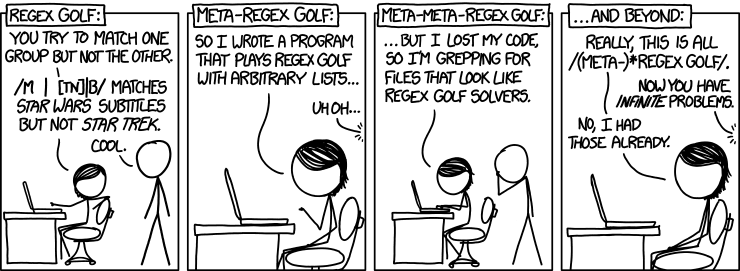
\includegraphics[width=.5\linewidth]{./gfx/19-xkcd-regex_golf}
\end{center}
\footnotesize
\emph{\rx{/bu|[rn]t|[coy]e|[mtg]a|j|iso|n[hl]|[ae]d|lev|sh|[lnd]i|[po]o|ls/} matches the last names of elected US presidents but not their opponents.}

%\vspace{6pt}
Source: \url{https://xkcd.com/1313/}
%
\end{frame}

% =========================================================================== %

\end{document}

% MAREI!!
% whom do I give credit? Where?